%%%%%%%%%%%%%%%%%%%%%%%%%%%%%%%%%%%%%%%%%%%%%%%%%%%%%%%%%%%%%%%%%%%%%%%%%%%%%%%
%%%%%%%%%%%%%%%%%%%%%%%%%%%%%%%%%%%%%%%%%%%%%%%%%%%%%%%%%%%%%%%%%%%%%%%%%%%%%%%
%%%%%%%%%%%%%%%%%%%%%%%%%%%%%%%%%%%%%%%%%%%%%%%%%%%%%%%%%%%%%%%%%%%%%%%%%%%%%%%
%%%%%%%%%%%%%%%%%%%%%%%%%%%%%%%%%%%%%%%%%%%%%%%%%%%%%%%%%%%%%%%%%%%%%%%%%%%%%%%
\section{Inferring Spatial Proximity Networks}
%%%%%%%%%%%%%%%%%%%%%%%%%%%%%%%%%%%%%%%%%%%%%%%%%%%%%%%%%%%%%%%%%%%%%%%%%%%%%%%
%%%%%%%%%%%%%%%%%%%%%%%%%%%%%%%%%%%%%%%%%%%%%%%%%%%%%%%%%%%%%%%%%%%%%%%%%%%%%%%
%%%%%%%%%%%%%%%%%%%%%%%%%%%%%%%%%%%%%%%%%%%%%%%%%%%%%%%%%%%%%%%%%%%%%%%%%%%%%%%
%%%%%%%%%%%%%%%%%%%%%%%%%%%%%%%%%%%%%%%%%%%%%%%%%%%%%%%%%%%%%%%%%%%%%%%%%%%%%%%
The network interference was driven by a combination of an exploratory data analysis and an iterative pipeline development process.
It serves as a prerequisite for the network analysis part of this thesis.
To generate functional and non-functional requirements of the pipeline, I conducted an analysis of the tracking data and a literature review, presented in section~\ref{ch:relatedwork}.
The analysis led to a general understanding of the data, its structure, characteristics and an estimation of its quality.
The purpose of the literature review was to get an overview of the common methods and approaches regarding network analysis in the field behavioral insect studies.

Both results are then used to select a network type and to define its nodes and links.
Furthermore, I inferred specific pipeline parameters and decided for the procedure of network extraction.
The pipeline was developed, tested and refined in an iterative process.
Accordingly, the results of the evaluation lead to new or changing functional requirements.
The evaluation is conducted by reviewing the pipeline parameters' effects on network properties and checking the validity and quality of the networks by investigating the age of bees in the resulting network.

%%%%%%%%%%%%%%%%%%%%%%%%%%%%%%%%%%%%%%%%%%%%%%%%%%%%%%%%%%%%%%%%%%%%%%%%%%%%%%%
%%%%%%%%%%%%%%%%%%%%%%%%%%%%%%%%%%%%%%%%%%%%%%%%%%%%%%%%%%%%%%%%%%%%%%%%%%%%%%%
\subsection{Defining the Network and its Parameters}
%%%%%%%%%%%%%%%%%%%%%%%%%%%%%%%%%%%%%%%%%%%%%%%%%%%%%%%%%%%%%%%%%%%%%%%%%%%%%%%
%%%%%%%%%%%%%%%%%%%%%%%%%%%%%%%%%%%%%%%%%%%%%%%%%%%%%%%%%%%%%%%%%%%%%%%%%%%%%%%
As this work constitutes the first step towards network analysis using this tracking data I chose to infer a time-aggregated spatial proximity network.
Accordingly, the interactions are undirected but weighted.
Methods for analyzing static networks are widely established.
Static tools and algorithms are already implemented and used by a large community.
The results of the network analysis are easy to understand and interpret.
Additionally, static networks are the precondition for applying traditional community detection algorithms. My choice also establishes the comparability with \textcite{mersch2013tracking}.

Each node in the network represents a bee, identified by an ID.
The network consists only of bees that interact with other bees at least once, during the specified time interval.

Two bees are associated (spatially close to each other) if their distance is smaller than a \emph{maximum distance}.
Using only this criterion leads to many interactions, resulting in a very dense network, because an interaction could only last for 0.33 seconds.
Therefore, an additional parameter, the \emph{minimum contact duration}, is introduced.
It specifies the minimum time two bees have to spend close to each other to be called associated.

Links are assigned two attributes.
The first one is the frequency of contacts, meaning how often they share a close position. The second parameter refers to the total duration of all contacts.

The network pipeline takes two types of parameters. The first set of parameters defines the resulting network and the exact type of spatial proximity. The second set relates to the given data set. Both parameter types are described below.

\begin{table}[htbp]
\small
\centering
\begin{tabularx}{\textwidth}{@{} r Y @{}}
\textbf{Maximum distance} & Level of closeness between to individual bees.~(in pixel) \vspace{2mm} \\
\textbf{Minimum} & The number of frames two individuals need to spend close.\\
\textbf{Contact duration} &  to each other to count it as an interaction ~(in frames) \vspace{2mm} \\
\textbf{Start timestamp} & Starting point of the network aggregation.~(as UTC string) \vspace{2mm} \\
\textbf{Window size} & Size of time window for aggregating the network.~(in minutes) \vspace{6mm}\\
\textbf{Confidence} & Level of confidence, as described in section~\nameref{subsec:confidence}.~(in percent) \vspace{2mm}\\
\textbf{Valid IDs} & List of valid IDs within a specified time interval, as described in section~\nameref{subsubsec:dataset:filter}.~(in CSV file format) \vspace{2mm}\\
\textbf{Gap Size} & Gaps in time series of bee pairs are assumed to be the result of missing detections. Gaps of this size are filled up.~(in frames)\vspace{2mm}\\
\textbf{Number of CPUs} & Number of used CPUs for parallelization. \vspace{2mm}\\
\textbf{Year} & Calculate bee IDs and stitching of camera images according to the observation period.~(2015 or 2016)\\
\end{tabularx}
\end{table}

%%%%%%%%%%%%%%%%%%%%%%%%%%%%%%%%%%%%%%%%%%%%%%%%%%%%%%%%%%%%%%%%%%%%%%%%%%%%%%%
%%%%%%%%%%%%%%%%%%%%%%%%%%%%%%%%%%%%%%%%%%%%%%%%%%%%%%%%%%%%%%%%%%%%%%%%%%%%%%%
\subsection{Choosing Parameter Values for Network Analysis}
%%%%%%%%%%%%%%%%%%%%%%%%%%%%%%%%%%%%%%%%%%%%%%%%%%%%%%%%%%%%%%%%%%%%%%%%%%%%%%%
%%%%%%%%%%%%%%%%%%%%%%%%%%%%%%%%%%%%%%%%%%%%%%%%%%%%%%%%%%%%%%%%%%%%%%%%%%%%%%%
For network analysis, I chose three days: 20 August, 22 August, and 24. August.
These days were selected because bees from a wide range of age groups were present and older bees, which are likely to be foragers, were more represented in the hive during these days.
Additionally, no data is missing due to camera failures.
The following values are chosen according to biological constraints and similar to other studies, for better comparability.

I chose the length of a bee body, according to \textcite{baracchi2014socio}, as the maximum distance between two bees (Figure~\ref{fig:contactRadius}).
The average bee length of $212$px ($\pm 16$px)  was determined by manually measuring the length of all bees ($n=337$) in images from the four cameras using the tool ImageJ\footnote{\url{http://imagej.net/Welcome}; Last accessed:
 22.02.2016}.
The minimum contact duration is set to three frames (one second). This value corresponds to~\textcite{mersch2013tracking}, as they also exclude interactions below one second.
The networks are aggregated for ten hours during daylight; this corresponds to the biological rhythm of bees.

The confidence level is set to $95\%$, which will keep about 60\% of the data.
The gap size is set to two frames. This value corresponds to the median gap length in the time series of bee pairs.

\begin{table}[htbp]
\small
\centering
\caption[Parameters chosen for network analysis]{\textbf{Parameters chosen for network analysis} The maximum distance corresponds to the length of a bee body and the minimum contact duration is about one second. The networks are aggregated for ten hours.\\
}
\label{tab:chosenparams}

\begin{tabular}{rrl}
	\toprule
	\textbf{Parameter} & \textbf{Value} & \textbf{Unit} \\ \midrule
	Maximum distance & 212 & px \\
	Minimum contact duration & 3 & frames \\
	Window size & 600 & minutes \\ \midrule
	Confidence & 95 & percent \\
	Gap size & 2 & frames \\
	\bottomrule
\end{tabular}

\end{table}

\begin{figure}[bp]
	\centering
	\begin{subfigure}[b]{0.45\textwidth}
		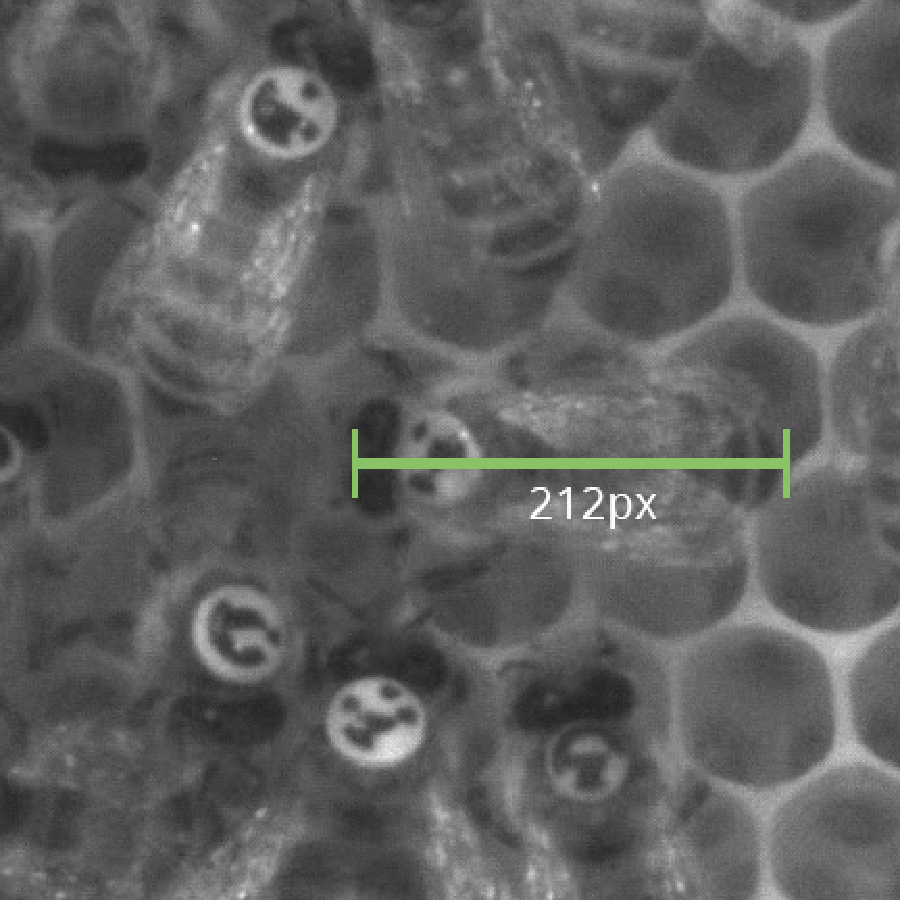
\includegraphics[width=\textwidth]{Figures/sizeTagBee}
		\caption[Body length of a bee]{Body length of a bee}
		\label{fig:size}
	\end{subfigure}
	\hspace{0.08\textwidth}
	\begin{subfigure}[b]{0.45\textwidth}
		\centering
		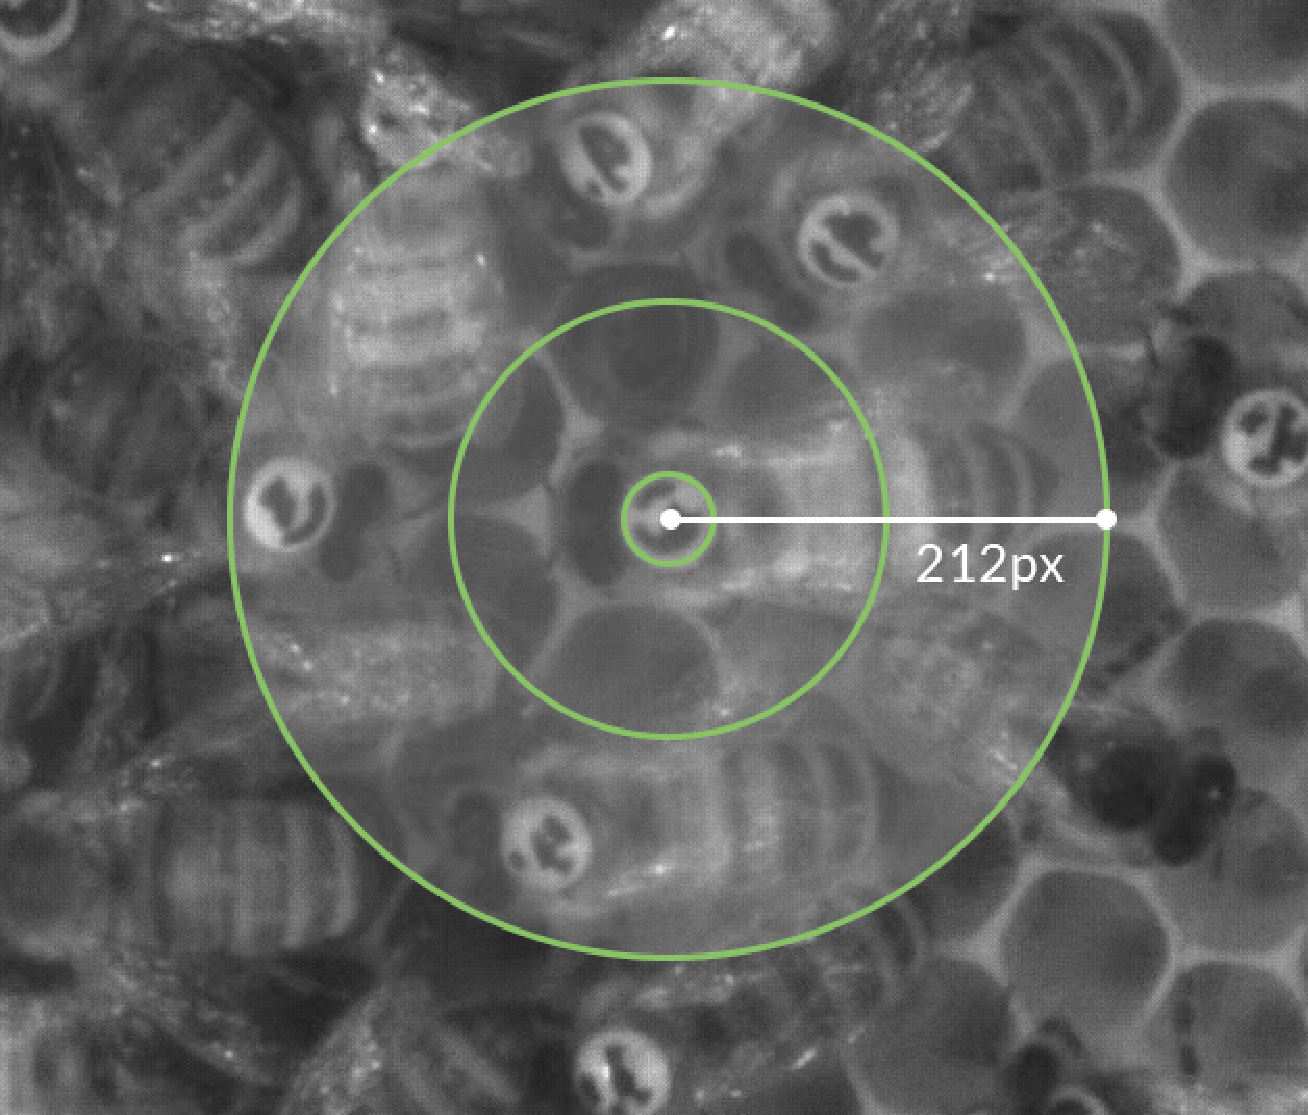
\includegraphics[width=\textwidth]{Figures/radius}
		\caption[Contact radius]{Contact radius}
		\label{fig:radius}
	\end{subfigure}
	\caption[Maximum distance of bees]{\textbf{Maximum distance of bees}: A length of a bee body is chosen as the maximum distance between two bees.}
	\label{fig:contactRadius}
\end{figure}


%%%%%%%%%%%%%%%%%%%%%%%%%%%%%%%%%%%%%%%%%%%%%%%%%%%%%%%%%%%%%%%%%%%%%%%%%%%%%%%
%%%%%%%%%%%%%%%%%%%%%%%%%%%%%%%%%%%%%%%%%%%%%%%%%%%%%%%%%%%%%%%%%%%%%%%%%%%%%%%
\subsection{Summary}
%%%%%%%%%%%%%%%%%%%%%%%%%%%%%%%%%%%%%%%%%%%%%%%%%%%%%%%%%%%%%%%%%%%%%%%%%%%%%%%
%%%%%%%%%%%%%%%%%%%%%%%%%%%%%%%%%%%%%%%%%%%%%%%%%%%%%%%%%%%%%%%%%%%%%%%%%%%%%%%
The goal, as mentioned in~\ref{sec:intro:goals}, was to answer the question whether it is possible to infer temporal networks with the provided honey bee tracking data and to work out challenges and limitations regarding the provided data set. Furthermore, it was a goal to identify the parameters necessary for the pipeline.

\subsubsection{Pipeline Parameters}
%%%%%%%%%%%%%%%%%%%%%%%%%%%%%%%%%%%%%%%%%%%%%%%%%%%%%%%%%%%%%%%%%%%%%%%%%%%%%%%
This analysis results in two types of pipeline parameters. The first category specifies the resulting network, concerning the definition of spatial proximity, duration of interaction and size of the aggregated time window. The second type represents parameters resulting out of the characteristics of the dataset.

\begin{enumerate}
\item \textbf{Pipeline parameters for network}\\
maximum distance, minimum contact duration, window size
\item \textbf{Pipeline parameters for data}\\
confidence, list of valid IDs, gap size
\end{enumerate}


\subsubsection{Limitations}
%%%%%%%%%%%%%%%%%%%%%%%%%%%%%%%%%%%%%%%%%%%%%%%%%%%%%%%%%%%%%%%%%%%%%%%%%%%%%%%
It is possible to infer networks, but a complex preprocessing of the dataset is essential with two major steps:

\begin{enumerate}
\item \textbf{Reduction of data}\\
Reduce the amount of data to obtain a reliable data set, by filtering out detections with a low confidence value or by IDs with a low detection frequency.
\item \textbf{Combine camera data}\\
This step consist of the time synchronization of each of the two cameras and the joining of the data per frame.
\end{enumerate}

A tradeoff exists between the remaining amount of data that can be used for network inference and the data's.
A high confidence value reduces the amount of data and produces gaps.
The gap size parameter tries to fix this problem. 

It is also possible to infer time-aggregated networks, but with restrictions.
When limiting the window size for network aggregation to the biological rhythms of day and night\footnote{Any other window size entails the inclusion of the duration of biological processes related to honey bees, I would need to know beforehand. Alternatively, I would need to apply a method to infer an appropriate window size out of the given data, this it out of scope.}, only a small amount of useful analysis days remain due to a large number of interruptions.